\documentclass[a4paper]{article}

\usepackage[bindingoffset=0.2in,left=1.2in,right=1.2in,top=1.2in,bottom=1in,footskip=.25in]{geometry}
% deutsche Silbentrennung
\usepackage[ngerman]{babel}
% wegen deutschen Umlauten
\usepackage[utf8]{inputenc}
\usepackage[T1]{fontenc}
\usepackage{amsmath}
\usepackage{graphicx}
\usepackage{float}
\usepackage{epstopdf}
\usepackage[colorinlistoftodos]{todonotes}
\usepackage{url}
\usepackage{tikz}
\usetikzlibrary{calc}
\usepackage[hidelinks]{hyperref}
\usepackage{subcaption}
\usepackage{verbatim}
\usepackage{pgfplots}
\pgfplotsset{compat=1.9}
\usepackage{listings}
\usepackage{textcomp}
\usepackage{bbold}
\usepackage{mathtools} 

\lstset{basicstyle=\footnotesize\ttfamily,language={}}
\newcommand{\textapprox}{\raisebox{0.5ex}{\texttildelow}}
\newcommand\numberthis{\addtocounter{equation}{1}\tag{\theequation}}
\graphicspath{{./graphics/}}

\title{PR Computational Physics 2014W \\ Ereignisbasierte Molekulardynamik-Simulation von Harten Kugeln}

\author{
	Maud Formanek, 0909317\\
    \texttt{maud.formanek@univie.ac.at}
	\and
    Abraham Hinteregger,  1025914\\
    \texttt{abraham.hinteregger@univie.ac.at}\and
    Patrick Derflinger,  1008451\\
    \texttt{a1008451@unet.univie.ac.at}
    }
\date{\today}

\newcommand{\TODO}[1][\!\!]{\textcolor{red}{TODO #1}}


\begin{document}
\maketitle
\tableofcontents

\newpage

\section{Einführung} \label{einfuehrung}
% !TeX root = ../Harte_Kugeln.tex
Ziel dieser im Rahmen des Praktikums ``Computational Physics'' im Wintersemester 2014 unter der Aufsicht von Prof. Martin Neumann angefangenen Arbeit war es, eine ereignisbasierte Molekulardynamik zur Simulation eines Systems von harten Kugeln zu implementieren. Im ersten Teil dieser Arbeit wird die Motivation der Methode sowie Details bezüglich der Kollisionsberechnung und -Behandlung erläutert. Anschließend werden Ergebnisse der Simulation präsentiert. Untersucht wurden in diesem Fall die Paarverteilungsfunktion bei verschiedenen Aggregatszuständen, die thermische Zustandsgleichung, die Diffusionskonstante sowie die Verteilung der freien Bewegungszeiten (Zeitdifferenz zweier Stöße).
% !TeX root = ../Harte_Kugeln.tex
\section{Methode }
%\TODO[überschriften vllt anpassen]
Harte Kugeln sind ein vereinfachtes Modell für die Interaktion zwischen Molekülen bei der angenommen wird, dass Moleküle runde Objekte (Kugeln) sind, welche nur durch elastische Stöße miteinander wechselwirken.
Dass die Stöße elastisch sind, bedeutet, dass keine Energie durch Zustandsänderung der Kugeln zugeführt wird oder verloren geht. Es findet also weder Deformation noch Erwärmung der Kugeln statt und auch der Drehimpuls spielt keine Rolle. Die Kugeln bewegen sich daher frei mit konstantem Impuls und konstanter Energie, bis sie auf eine andere Kugel --- oder bei nicht periodischen Randbedingungen auf die Grenze der Simulation --- stoßen. Das Potential eines derartigen Moleküls ist in Abb. \ref{fig:hkpotential} dargestellt.
\begin{figure}[H] \centering
\begin{tikzpicture}
	\begin{axis}[
		xlabel=$r$,
		xtick={0,2,8},
		 xticklabels={$0$,$R$,$\infty$},
		 ytick={0,10},
		 yticklabels={$0$,$\infty$},
		ylabel={$U(r) = \delta(r-R)$}
	]
%\addplot+[color=blue,thick] coordinates { (0,2) (2,2)  (2,0) (9,0) }; % + wegmachen wenn punkte stören
\addplot[color=red] coordinates { (0,10) (2,10) (2,10) (2,0) (9,0) };    % auskommentieren je nachdem welcher plot besser ist (ggfs Achse anpassen)
\end{axis}
\end{tikzpicture}
\caption{Potential einer harten Kugel mit Radius $R$ auf Teilchen (infinitesimal kleine) im Abstand $r$}
 \label{fig:hkpotential}
\end{figure} 
\subsection{Ereignisbasierte Molekulardynamik}

Im Gegensatz zur herkömmlichen Molekulardynamik, bei der die Bewegung der Moleküle aus Integration der wirkenden Kräfte mit einem konstanten Zeitschritt folgt, wird bei der ereignisbasierten Molekulardynamik eine Liste über alle (zumindest alle relevanten) in der Zukunft liegenden Stöße geführt. Nach jedem Stoß wird die Zeit bis zum nächsten Stoß ``vorgespult'', eine Kollision berechnet und die Liste aktualisiert.

%Das untersuchte System war eine Box mit periodischen Randbedingungen gefüllt mit harten Kugeln (\ref{sec:hk})

Die Motivation der Methode ist, dass bei herkömmlicher MD (Molekulardynamik) mit konstantem Zeitschritt zwischen zwei Stößen viele unnötige Berechnungen durchgeführt werden. Wenn man den Zeitschritt größer macht würde sich diese Anzahl zwar senken, dafür hätte man bei Stößen das Problem, dass sich eine Kugel innerhalb eines Zeitschritts in eine andere hinein bewegen könnte, was dann entweder zu Ungenauigkeiten oder zusätzlichem Rechenaufwand (Zeit zurück drehen und mit kleineren Zeitschritten sondieren) führt.
% erweitern?

\subsection{Berechnung der Stöße}
\newcommand{\reffig}[1]{Abbildung \ref{fig:#1}}

Um die nächste Stoßzeit zu ermitteln genügt es, sich jeweils Zwei Kugeln anzusehen und sich deren Kollisionszeit zu berechnen. Weiß man die Kollisionszeiten aller Kugeln im System, so weiß man auch den Zeitpunkt der nächsten Kollision. Man muss also nicht das System als ganzes betrachten, es genügt das Verhalten von jeweils zwei Kugeln zu kennen.
Im Zentrum der Simulation steht somit der Algorithmus zur Erkennung ob und wann zwei Kugeln einander stoßen werden. 
Da wir eine Box mit periodischen Randbedingungen betrachten, muss der gewählte Algorithmus auch mit Kugeln am Rand der Box klarkommen. Unser Ansatz beruht auf einer Koordinatentransformation und wird in diesem Kapitel näher beschrieben.


% !TeX root = ../Harte_Kugeln.tex
\subsubsection{Kollisionsprüfung} % Probenentnahme? Messungsintervalle? 

%Parameter zur Darstellung der Box und Kugeln in diesem Absatz
\newcommand{\BoxW}{10}
\newcommand{\BoxH}{7}
\newcommand{\Kradius}{.7}

\newcommand{\Kx}{7}
\newcommand{\Ky}{6}

\newcommand{\vxa}{6/3}
\newcommand{\vya}{2/3}
\newcommand{\vxb}{-5/3}
\newcommand{\vyb}{3/3}

\newcommand{\Dx}{-2.5}
\newcommand{\Dy}{-5}

\newcommand{\BoxC}{\BoxW / 2 , \BoxH / 2}
\newcommand{\BoxWh}{\BoxW / 2}
\newcommand{\BoxHh}{\BoxH / 2}

\newcommand{\drawKugel}[1]{
    \draw[fill=black] 	(#1) circle (0.15em);
    \draw		(#1) circle (\Kradius);
}

\newcommand{\dis}{r_{21}}
\newcommand{\vdis}{\vec{r}_{21}}
\newcommand{\vdissq}{\left|\vdis\right|^2}

\newcommand{\vel}{v_{21}}
\newcommand{\vvel}{\vec{v}_{21}}
\newcommand{\vvelsq}{\left|\vvel\right|^2}
\newcommand{\dia}{d}

%\subsubsection{Koordinatentransformation}
Zur besseren Veranschaulichung wird der Algorithmus in 2 Dimensionen vorgestellt, er ist jedoch ohne Probleme auf beliebige Dimensionen erweiterbar.\\
In \reffig{Koortrans01} ist die Ausgangsposition zweier beliebiger Kugeln dargestellt. In dieser Darstellung ist eine Berechnung der Kollision erschwert da beide Kugeln ohne Kontakt und zu verschiedenen Zeiten die betrachtete Box verlassen.

% !TeX root = ../Harte_Kugeln.tex

\begin{figure}[H]
  \centering
  \begin{tikzpicture}
    \coordinate (Origin)   at (0,0);
    \coordinate (OL) at (0,\BoxH);
    \coordinate (OR) at (\BoxW,\BoxH);
    \coordinate (UR) at (\BoxW,0);
    
    \draw [very thick] (Origin) -- (OL) -- (OR) -- (UR) -- (Origin);
    
    \coordinate [label={below right:$K_2$}] (K2) at (\Kx,\Ky);
    \drawKugel{K2};
    
    \coordinate [label={below:$K_1$}] (K1) at (\Kx+\Dx,\Ky+\Dy);
    \drawKugel{K1};

	\draw[-latex, thick] (K2) -- (K1) node[midway,above,sloped] {$\vdis$};
	
	\draw[-latex, thick] (K1) -- (\Kx+\Dx+\vxa, \Ky+\Dy+\vya) node[midway,above,sloped] {$\vec{v}_1$};
	\draw[-latex, thick] (K2) -- (\Kx+\vxb, \Ky+\vyb) node[midway,above,sloped] {$\vec{v}_2$};
  \end{tikzpicture}
  \caption{Ausgansposition der betrachteten Kugeln.}
  \label{fig:Koortrans01}
\end{figure}





Um eine leichter zu handhabende Darstellung zu erhalten und Effekten mit Stoßpartnern am Rand unserer Box aus dem Weg zu gehen transformieren wir unser System so, dass sich eine der am berechneten Stoß beteiligten Kugeln im Zentrum der Box befindet. Da wir eine Box mit periodischen Randbedingungen gewählt haben ist dies ohne weitere Probleme möglich. In \reffig{Koortrans02} ist das Resultat einer solchen Verschiebung um Kugel 2 zu sehen.

% !TeX root = ../Harte_Kugeln.tex

\begin{figure}[H]
  \centering
  \begin{tikzpicture}
    \coordinate (Origin)   at (0,0);
    \coordinate (OL) at (0,\BoxH);
    \coordinate (OR) at (\BoxW,\BoxH);
    \coordinate (UR) at (\BoxW,0);
    
    \draw [very thick] (Origin) -- (OL) -- (OR) -- (UR) -- (Origin);
    
    \coordinate [label={below right:$K_2$}] (K2) at (\BoxC);
    \drawKugel{K2};
    
    \coordinate [label={below:$K_1$}] (K1) at (\BoxWh+\Dx,\BoxHh+\Dy);
    \drawKugel{K1};
    
	\draw[-latex, thick] (K2) -- (K1) node[midway,above,sloped] {$\vdis$};
	
	\draw[-latex, thick] (K1) -- (\BoxWh+\Dx+\vxa, \BoxHh+\Dy+\vya) node[midway,above,sloped] {$\vec{v}_1$};
	\draw[-latex, thick] (K2) -- (\BoxWh+\vxb, \BoxHh+\vyb) node[midway,above,sloped] {$\vec{v}_2$};
  \end{tikzpicture}
  \caption{Koordinatentransformation Kugel 2 ins Zentrum der Box.}
  \label{fig:Koortrans02}
\end{figure}

Da es durch die Verschiebung dazu kommen kann, dass Kugel 1 die betrachtete Box verlässt, wie in \reffig{Koortrans03} zu sehen, muss sie durch Anwendung der Randbedingungen wieder in die Box gelegt werden.

% !TeX root = ../Harte_Kugeln.tex

\begin{figure}[H]
  \centering
  \begin{tikzpicture}
    \coordinate (Origin)   at (0,0);
    \coordinate (OL) at (0,\BoxH);
    \coordinate (OR) at (\BoxW,\BoxH);
    \coordinate (UR) at (\BoxW,0);
    
    \draw [very thick] (Origin) -- (OL) -- (OR) -- (UR) -- (Origin);
    
    \coordinate [label={below:$K_2$}] (K2) at (\BoxC);
    \drawKugel{K2};
    
    \coordinate [label={below:$K_1$}] (K1) at (\BoxWh+\Dx,\BoxHh+\Dy+\BoxH);
    \drawKugel{K1};
    
	\draw[-latex, thick] (K2) -- (K1) node[midway,above,sloped] {$\vdis$};
	
	\draw[-latex, thick] (K1) -- (\BoxWh+\Dx+\vxa, \BoxHh+\Dy+\BoxH+\vya) node[midway,above,sloped] {$\vec{v}_1$};
	\draw[-latex, thick] (K2) -- (\BoxWh+\vxb, \BoxHh+\vyb) node[midway,below,sloped] {$\vec{v}_2$};
  \end{tikzpicture}
  \caption{Kugel 1 wieder in die Box zurück gesetzt.}
  \label{fig:Koortrans03}
\end{figure}

Es ist nur Relativgeschwindigkeit der beiden Kugeln entscheidend und daher kann die Kugel im Zentrum als in Ruhe betrachten, solange sich die andere Kugeln mit der Relativgeschwindigkeit $\vvel=\vec{v}_1-\vec{v}_2$ bewegt.
 
% !TeX root = ../Harte_Kugeln.tex

\begin{figure}[H]
  \centering
  \begin{tikzpicture}
    \coordinate (Origin)   at (0,0);
    \coordinate (OL) at (0,\BoxH);
    \coordinate (OR) at (\BoxW,\BoxH);
    \coordinate (UR) at (\BoxW,0);
    
    \draw [very thick] (Origin) -- (OL) -- (OR) -- (UR) -- (Origin);
    
    \coordinate [label={below:$K_2$}] (K2) at (\BoxC);
    \drawKugel{K2};
    
    \coordinate [label={below:$K_1$}] (K1) at (\BoxWh+\Dx,\BoxHh+\Dy+\BoxH);
    \drawKugel{K1};
    
	\draw[-latex, thick] (K2) -- (K1) node[midway,above,sloped] {$\vdis$};
	
	\draw[-latex, thick] (K1) -- (\BoxWh+\Dx+\vxa-\vxb, \BoxHh+\Dy+\BoxH+\vya-\vyb) node[midway,above,sloped] {$\vvel$};
  \end{tikzpicture}
  \caption{Relativgeschwindigkeit auf Kugeln 1 übertragen.}
  \label{fig:Koortrans04}
\end{figure}

Hat man nun eine Darstellung wie in \reffig{Koortrans04} vorliegen, so kann man die Kollisionszeit durch Anwendung simpler Geometrie erhalten.
Es gilt die Abstandsgleichung 
\begin{equation}
	\vec{x} = \vdis + t\cdot\vvel
\end{equation}
mit 
\begin{equation}
	\left|\vec{x}\right| \overset{!}{=} \dia \Rightarrow \left|x\right|^2 = \dia^2
\end{equation}
zu lösen, wobei $\dia=\sigma_1/2 + \sigma_2/2$ gilt.

Somit erhält man
\begin{align}
	\dia^2	&= \left(\vdis + t\cdot\vvel \right)^2 \\
			&= \vdissq + 2t\cdot\vdis\cdot\vvel + t^2\vvelsq
\end{align}
und nach Auflösen nach der Kollisionszeit $t$
\begin{equation}
	t_{1,2}=\frac{\vdis\cdot\vvel \pm \sqrt{\left(\vdis\cdot\vvel\right)^2 - \vdissq\vvelsq + \vvelsq\dia^2}}{\vvelsq}.
\end{equation}

Die Berechnung kann noch vereinfacht werden. Wie man in \reffig{Koortrans04} sieht, kann es nur zu einer Kollision kommen wenn $\vdis\cdot\vvel < 0$ ist. Daher kann nur die Addition des Wurzelterms zu einem Ergebnis mit positiver Zeit führen.\\
Kommt es zu keinem Stoß in dieser Box, so verlässt Kugel 1 die Box und wird, entsprechend den Randbedingungen des Systems, wieder zurückgesetzt.


\subsubsection{Berechnung der Impulsänderung durch Stöße}
Der Berechnung der Stöße liegt die Erhaltung von Impuls und Energie zugrunde. Wenn zwei Kugeln mit Massen $m_1,m_2$ und Geschwindigkeiten $v_1,v_2$ aufeinandertreffen verlassen verändern sich die Geschwindigkeiten zu $v_1'$ und $v_2'$.
\begin{align*}
m_1v_1 + m_2v_2 &= m_1v_1'+m_2v_2'\\
\frac{m_1v^2_1}{2}\frac{m_2v^2_2}{2} &= \frac{m_1v'^2_1}{2}\frac{m_2v'^2_2}{2}
\end{align*}
\\
Da bei einem Stoß nur eine Kraft normal auf die Kugeln (parallel zum Vektor $\vec r_{12} = \vec r_2 - \vec r_1$  zwischen den beiden Kugelmittelpunkten $\vec r_i, i\in \{1,2\}$ wirkt ist auch nur die entsprechende Komponente der Geschwindigkeit betroffen.\\
Aus den Erhaltungssätzen und dieser Überlegung lässt sich dann das Verhalten der Kugeln bei einem Stoß herleiten:
\begin{align*}
\vec v_1' &= \vec v_1 + \Delta \vec v\\
\vec v_2'& = \vec v_2 - \Delta \vec v\\
\Delta\vec v &= \left(\vec r_2 - \vec r_1\right) \cdot \left(\vec v_2 - \vec v_1\right)\frac{\left(\vec r_2 - \vec r_1\right)}{R^2}
\end{align*}

\begin{figure}[H] \centering
\begin{tikzpicture}
\draw[white] (-1,-1.75) rectangle(2.5,2.5);
  \shade[ball color=gray!10!] (0,0) coordinate(A) circle (0.77) ;
  \draw[orange,fill=orange, opacity=0.5] (0.8,-1,1.3) -- ++(0,2,0) -- ++(0,0,-2) -- ++(0,-2,0) -- cycle;
  \shade[ball color=gray!10!] (1.6,0,0.6) coordinate(B) circle (0.8) ;
  \draw[thick,-latex,red] (A) --+ (0.55,1) node[right]{$\vec v_1$} ;
  \draw[thick,-latex,red] (B) --+ (-1.1,-1) node[left]{$\vec v_2$} ;
%  \draw (4,.2) node[right]{H$^-$} ;
  \foreach \point in {A,B}
  	\fill [black] (\point) circle (1pt) ;
\end{tikzpicture} \hfill
\begin{tikzpicture}
\draw[white] (-1,-1.75) rectangle(2.5,2.5);


  \shade[ball color=gray!10!] (0,0) coordinate(A) circle (0.8) ;
  \shade[ball color=gray!10!] (1.6,0) coordinate(B) circle (0.8) ;
  \draw[very thick, orange, opacity=0.5](0.8,-0.8) --+(0,1.6);
  \draw[thick,-latex,red] (A) --+ (0.5,1) node[right]{$\vec v_1$} ;
  \draw[thick,-latex,red] (B) --+ (-1,-1) node[left]{$\vec v_2$} ;
%  \draw (4,.2) node[right]{H$^-$} ;
  \foreach \point in {A,B}
  	\fill [black] (\point) circle (1pt) ;
\end{tikzpicture} \hfill
\begin{tikzpicture}
\draw[white] (-1,-1.75) rectangle(2.5,2.5);
  \shade[ball color=gray!10!] (0,0) coordinate(A) circle (0.8) ;
  \shade[ball color=gray!10!] (1.6,0) coordinate(B) circle (0.8) ;
    \draw[very thick, orange, opacity=0.5](0.8,-0.8) --+(0,1.6);
  \draw[thick,-latex,red!50!] (A) --+ (1.5,2) node[right]{$\vec v_1$} ;
  \draw[thick,-latex,blue] (A) --+ (0.96,2) node[right]{$\vec v_1'$} ;
  \draw[thick,-latex,blue] (B) --+ (0.53,0) node[above]{$\vec v_2'$} ;
%  \draw (4,.2) node[right]{H$^-$} ;
  \foreach \point in {A,B}
  	\fill [black] (\point) circle (1pt) ;
\end{tikzpicture} \hfill
\begin{tikzpicture}
\draw[white] (-1,-1.75) rectangle(2.5,2.5);
  \shade[ball color=gray!10!] (0,0) coordinate(A) circle (0.8) ;
  \shade[ball color=gray!10!] (1.6,0) coordinate(B) circle (0.8) ;
    \draw[very thick, orange, opacity=0.5](0.8,-0.8) --+(0,1.6);
  \draw[thick,-latex,blue] (A) --+ (-0.04,1) node[above]{$\vec v_1'$} ;
  \draw[thick,-latex,blue] (B) --+ (-0.47,-1) node[below]{$\vec v_2'$} ;
%  \draw (4,.2) node[right]{H$^-$} ;
  \foreach \point in {A,B}
  	\fill [black] (\point) circle (1pt) ;
\end{tikzpicture}
\caption{Stoß von 2 Kugeln in 3 Dimensionen (ganz links) kann auf 2 dimensionalen Fall reduziert werden (mitte links) bei dem eine Kugel vor dem Stoß ruht (mitte rechts). Geschwindigkeiten vor dem Stoß jeweils in rot, Geschwindigkeiten der Kugeln nach dem Stoß jeweils in blau }
 \label{fig:kugelnstoss}
\end{figure} 

%\section{Implementation} \label{implementation}
\section{Resultate} \label{resultate}
% !TeX root = ../Harte_Kugeln.tex
\subsection{Paarverteilungsfunktion}
Eine Flüssigkeit oder ein Gas mit rein additiven Paarwechselwirkungen kann durch die sogenannte Paarverteilungsfunktion --- manchmal auch Paarkorrelationsfunktion oder radiale Verteilungsfunktion --- $g(r)$ vollständig charakterisiert werden. Diese Funktion gibt Aufschluss über die kurzreichweitige Struktur des Fluids --- also seine Nahordnung. Sie beschreibt die Häufigkeit, mit der sich zwei Teilchen in einem gewissen Abstand $r$ voneinander entfernt befinden, bezogen auf die jeweilige Häufigkeit in einem idealen Gas. Die Paarverteilungsfunktion ist demnach gegeben durch
\begin{equation}
g(r) = \frac{1}{4\pi r^2 \rho} \langle \sum_{j\neq i} \delta(r-r_{ij}) \rangle
\end{equation}   
Da Fluide keine Fernordnung besitzen, muss die Paarverteilungsfunktion im limes $r \rightarrow \infty$ gegen 1 konvergieren. Des weiteren sei angemerkt, dass die Paarverteilungsfunktion der Randverteilung der $N$-Teilchen-Wahrscheinlichkeitsdichte entspricht und man demnach im limes $\rho \rightarrow 0$ direkt das Paarpotential $U(r)$ aus der Paarverteilungsfunktion ablesen kann.  
\begin{equation}
\lim_{\rho \rightarrow 0} g(r) = e^{-\beta U(r)}
\end{equation}
Für Festkörper lässt sich natürlich auch eine Paarverteilungsfunktion definieren, allerdings ist diese nicht mehr isotrop sondern richtungsabhängig. 
\begin{equation}
g(\vec{r}) = \frac{1}{\rho N} \langle \sum_{j\neq i} \delta^{(3)}(\vec{r}-\vec{r_{ij}}) \rangle
\end{equation} 
Häufig wird aber auch die winkelgemittelte Version verwendet, welche dann mit der Definition der Paarverteilungsfunktion für Fluide übereinstimmt. 

Abbildungen \ref{fig:paarverteilung1}, \ref{fig:paarverteilung2} und \ref{fig:paarverteilung3} zeigen die Paarverteilungsfunktionen des Systems von Harte Kugeln für verschiedene Dichten $\rho$ von 0.2 bis 1.3. Die Entstehung von Nahordnung beim Übergang vom gasförmigen zum flüssigen Zustand mit zunehmender Dichte lässt sich gut anhand von Abbildung \ref{fig:paarverteilung1} erkennen. Im ungeordneten (gasförmigen) Zustand nimmt die Paarverteilungsfunktion mit der Entfernung monoton ab, während sich beim Phasenübergang zur Flüssigkeit ein zweites Maximum ausbildet. 
\begin{figure}[H]
 \centering
 \resizebox{0.9\textwidth}{!}{% GNUPLOT: LaTeX picture with Postscript
\begingroup
  \makeatletter
  \providecommand\color[2][]{%
    \GenericError{(gnuplot) \space\space\space\@spaces}{%
      Package color not loaded in conjunction with
      terminal option `colourtext'%
    }{See the gnuplot documentation for explanation.%
    }{Either use 'blacktext' in gnuplot or load the package
      color.sty in LaTeX.}%
    \renewcommand\color[2][]{}%
  }%
  \providecommand\includegraphics[2][]{%
    \GenericError{(gnuplot) \space\space\space\@spaces}{%
      Package graphicx or graphics not loaded%
    }{See the gnuplot documentation for explanation.%
    }{The gnuplot epslatex terminal needs graphicx.sty or graphics.sty.}%
    \renewcommand\includegraphics[2][]{}%
  }%
  \providecommand\rotatebox[2]{#2}%
  \@ifundefined{ifGPcolor}{%
    \newif\ifGPcolor
    \GPcolortrue
  }{}%
  \@ifundefined{ifGPblacktext}{%
    \newif\ifGPblacktext
    \GPblacktextfalse
  }{}%
  % define a \g@addto@macro without @ in the name:
  \let\gplgaddtomacro\g@addto@macro
  % define empty templates for all commands taking text:
  \gdef\gplbacktext{}%
  \gdef\gplfronttext{}%
  \makeatother
  \ifGPblacktext
    % no textcolor at all
    \def\colorrgb#1{}%
    \def\colorgray#1{}%
  \else
    % gray or color?
    \ifGPcolor
      \def\colorrgb#1{\color[rgb]{#1}}%
      \def\colorgray#1{\color[gray]{#1}}%
      \expandafter\def\csname LTw\endcsname{\color{white}}%
      \expandafter\def\csname LTb\endcsname{\color{black}}%
      \expandafter\def\csname LTa\endcsname{\color{black}}%
      \expandafter\def\csname LT0\endcsname{\color[rgb]{1,0,0}}%
      \expandafter\def\csname LT1\endcsname{\color[rgb]{0,1,0}}%
      \expandafter\def\csname LT2\endcsname{\color[rgb]{0,0,1}}%
      \expandafter\def\csname LT3\endcsname{\color[rgb]{1,0,1}}%
      \expandafter\def\csname LT4\endcsname{\color[rgb]{0,1,1}}%
      \expandafter\def\csname LT5\endcsname{\color[rgb]{1,1,0}}%
      \expandafter\def\csname LT6\endcsname{\color[rgb]{0,0,0}}%
      \expandafter\def\csname LT7\endcsname{\color[rgb]{1,0.3,0}}%
      \expandafter\def\csname LT8\endcsname{\color[rgb]{0.5,0.5,0.5}}%
    \else
      % gray
      \def\colorrgb#1{\color{black}}%
      \def\colorgray#1{\color[gray]{#1}}%
      \expandafter\def\csname LTw\endcsname{\color{white}}%
      \expandafter\def\csname LTb\endcsname{\color{black}}%
      \expandafter\def\csname LTa\endcsname{\color{black}}%
      \expandafter\def\csname LT0\endcsname{\color{black}}%
      \expandafter\def\csname LT1\endcsname{\color{black}}%
      \expandafter\def\csname LT2\endcsname{\color{black}}%
      \expandafter\def\csname LT3\endcsname{\color{black}}%
      \expandafter\def\csname LT4\endcsname{\color{black}}%
      \expandafter\def\csname LT5\endcsname{\color{black}}%
      \expandafter\def\csname LT6\endcsname{\color{black}}%
      \expandafter\def\csname LT7\endcsname{\color{black}}%
      \expandafter\def\csname LT8\endcsname{\color{black}}%
    \fi
  \fi
  \setlength{\unitlength}{0.0500bp}%
  \begin{picture}(8502.00,6802.00)%
    \gplgaddtomacro\gplbacktext{%
      \csname LTb\endcsname%
      \put(946,704){\makebox(0,0)[r]{\strut{} 0.8}}%
      \put(946,1537){\makebox(0,0)[r]{\strut{} 1}}%
      \put(946,2371){\makebox(0,0)[r]{\strut{} 1.2}}%
      \put(946,3204){\makebox(0,0)[r]{\strut{} 1.4}}%
      \put(946,4037){\makebox(0,0)[r]{\strut{} 1.6}}%
      \put(946,4870){\makebox(0,0)[r]{\strut{} 1.8}}%
      \put(946,5704){\makebox(0,0)[r]{\strut{} 2}}%
      \put(946,6537){\makebox(0,0)[r]{\strut{} 2.2}}%
      \put(1078,484){\makebox(0,0){\strut{} 1}}%
      \put(2483,484){\makebox(0,0){\strut{} 1.5}}%
      \put(3889,484){\makebox(0,0){\strut{} 2}}%
      \put(5294,484){\makebox(0,0){\strut{} 2.5}}%
      \put(6700,484){\makebox(0,0){\strut{} 3}}%
      \put(8105,484){\makebox(0,0){\strut{} 3.5}}%
      \put(176,3620){\rotatebox{-270}{\makebox(0,0){\strut{}$g(r)$}}}%
      \put(4591,154){\makebox(0,0){\strut{}$r [\text{m}]$}}%
    }%
    \gplgaddtomacro\gplfronttext{%
      \csname LTb\endcsname%
      \put(7118,6364){\makebox(0,0)[r]{\strut{}$\rho$ = 0.2}}%
      \csname LTb\endcsname%
      \put(7118,6144){\makebox(0,0)[r]{\strut{}$\rho$ = 0.3}}%
      \csname LTb\endcsname%
      \put(7118,5924){\makebox(0,0)[r]{\strut{}$\rho$ = 0.4}}%
      \csname LTb\endcsname%
      \put(7118,5704){\makebox(0,0)[r]{\strut{}$\rho$ = 0.5}}%
    }%
    \gplbacktext
    \put(0,0){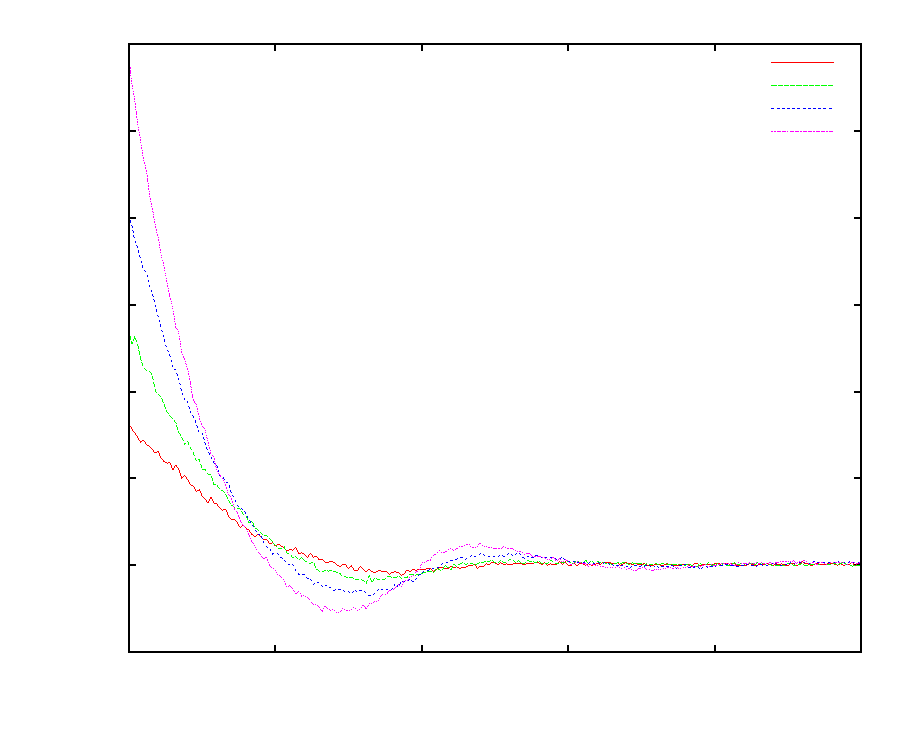
\includegraphics{PairDistribution1}}%
    \gplfronttext
  \end{picture}%
\endgroup
}
 \caption{Paarverteilungsfunktion für verschiedene Dichten $\rho$ im Bereich von 0.2 bis 0.5 (fluid)}
 \label{fig:paarverteilung1}
\end{figure} 

Harte Kugeln durchlaufen einen Phasenübergang vom flüssigen zum festen Zustand zwischen Packungsdichten von $n_f \approx 0.494$ und $n_s \approx 0.545$, was den reduzierten Dichten $\rho_f \approx 0.943$ und $\rho_s \approx 1.041$ entspricht. Anhand von Abbildungen \ref{fig:paarverteilung2} und \ref{fig:paarverteilung3} kann man diesen Phasenübergang deutlich erkennen --- die Maxima werden immer prominenter, was auf eine geordnete Kristallstruktur schließen lässt. 
 
\begin{figure}[H]
 \centering
 \resizebox{0.9\textwidth}{!}{% GNUPLOT: LaTeX picture with Postscript
\begingroup
  \makeatletter
  \providecommand\color[2][]{%
    \GenericError{(gnuplot) \space\space\space\@spaces}{%
      Package color not loaded in conjunction with
      terminal option `colourtext'%
    }{See the gnuplot documentation for explanation.%
    }{Either use 'blacktext' in gnuplot or load the package
      color.sty in LaTeX.}%
    \renewcommand\color[2][]{}%
  }%
  \providecommand\includegraphics[2][]{%
    \GenericError{(gnuplot) \space\space\space\@spaces}{%
      Package graphicx or graphics not loaded%
    }{See the gnuplot documentation for explanation.%
    }{The gnuplot epslatex terminal needs graphicx.sty or graphics.sty.}%
    \renewcommand\includegraphics[2][]{}%
  }%
  \providecommand\rotatebox[2]{#2}%
  \@ifundefined{ifGPcolor}{%
    \newif\ifGPcolor
    \GPcolortrue
  }{}%
  \@ifundefined{ifGPblacktext}{%
    \newif\ifGPblacktext
    \GPblacktextfalse
  }{}%
  % define a \g@addto@macro without @ in the name:
  \let\gplgaddtomacro\g@addto@macro
  % define empty templates for all commands taking text:
  \gdef\gplbacktext{}%
  \gdef\gplfronttext{}%
  \makeatother
  \ifGPblacktext
    % no textcolor at all
    \def\colorrgb#1{}%
    \def\colorgray#1{}%
  \else
    % gray or color?
    \ifGPcolor
      \def\colorrgb#1{\color[rgb]{#1}}%
      \def\colorgray#1{\color[gray]{#1}}%
      \expandafter\def\csname LTw\endcsname{\color{white}}%
      \expandafter\def\csname LTb\endcsname{\color{black}}%
      \expandafter\def\csname LTa\endcsname{\color{black}}%
      \expandafter\def\csname LT0\endcsname{\color[rgb]{1,0,0}}%
      \expandafter\def\csname LT1\endcsname{\color[rgb]{0,1,0}}%
      \expandafter\def\csname LT2\endcsname{\color[rgb]{0,0,1}}%
      \expandafter\def\csname LT3\endcsname{\color[rgb]{1,0,1}}%
      \expandafter\def\csname LT4\endcsname{\color[rgb]{0,1,1}}%
      \expandafter\def\csname LT5\endcsname{\color[rgb]{1,1,0}}%
      \expandafter\def\csname LT6\endcsname{\color[rgb]{0,0,0}}%
      \expandafter\def\csname LT7\endcsname{\color[rgb]{1,0.3,0}}%
      \expandafter\def\csname LT8\endcsname{\color[rgb]{0.5,0.5,0.5}}%
    \else
      % gray
      \def\colorrgb#1{\color{black}}%
      \def\colorgray#1{\color[gray]{#1}}%
      \expandafter\def\csname LTw\endcsname{\color{white}}%
      \expandafter\def\csname LTb\endcsname{\color{black}}%
      \expandafter\def\csname LTa\endcsname{\color{black}}%
      \expandafter\def\csname LT0\endcsname{\color{black}}%
      \expandafter\def\csname LT1\endcsname{\color{black}}%
      \expandafter\def\csname LT2\endcsname{\color{black}}%
      \expandafter\def\csname LT3\endcsname{\color{black}}%
      \expandafter\def\csname LT4\endcsname{\color{black}}%
      \expandafter\def\csname LT5\endcsname{\color{black}}%
      \expandafter\def\csname LT6\endcsname{\color{black}}%
      \expandafter\def\csname LT7\endcsname{\color{black}}%
      \expandafter\def\csname LT8\endcsname{\color{black}}%
    \fi
  \fi
  \setlength{\unitlength}{0.0500bp}%
  \begin{picture}(8502.00,6802.00)%
    \gplgaddtomacro\gplbacktext{%
      \csname LTb\endcsname%
      \put(946,704){\makebox(0,0)[r]{\strut{} 0.5}}%
      \put(946,1287){\makebox(0,0)[r]{\strut{} 1}}%
      \put(946,1871){\makebox(0,0)[r]{\strut{} 1.5}}%
      \put(946,2454){\makebox(0,0)[r]{\strut{} 2}}%
      \put(946,3037){\makebox(0,0)[r]{\strut{} 2.5}}%
      \put(946,3621){\makebox(0,0)[r]{\strut{} 3}}%
      \put(946,4204){\makebox(0,0)[r]{\strut{} 3.5}}%
      \put(946,4787){\makebox(0,0)[r]{\strut{} 4}}%
      \put(946,5370){\makebox(0,0)[r]{\strut{} 4.5}}%
      \put(946,5954){\makebox(0,0)[r]{\strut{} 5}}%
      \put(946,6537){\makebox(0,0)[r]{\strut{} 5.5}}%
      \put(1078,484){\makebox(0,0){\strut{} 1}}%
      \put(2483,484){\makebox(0,0){\strut{} 1.5}}%
      \put(3889,484){\makebox(0,0){\strut{} 2}}%
      \put(5294,484){\makebox(0,0){\strut{} 2.5}}%
      \put(6700,484){\makebox(0,0){\strut{} 3}}%
      \put(8105,484){\makebox(0,0){\strut{} 3.5}}%
      \put(176,3620){\rotatebox{-270}{\makebox(0,0){\strut{}$g(r)$}}}%
      \put(4591,154){\makebox(0,0){\strut{}$r [\text{m}]$}}%
    }%
    \gplgaddtomacro\gplfronttext{%
      \csname LTb\endcsname%
      \put(7118,6364){\makebox(0,0)[r]{\strut{}$\rho$ = 0.6}}%
      \csname LTb\endcsname%
      \put(7118,6144){\makebox(0,0)[r]{\strut{}$\rho$ = 0.7}}%
      \csname LTb\endcsname%
      \put(7118,5924){\makebox(0,0)[r]{\strut{}$\rho$ = 0.8}}%
      \csname LTb\endcsname%
      \put(7118,5704){\makebox(0,0)[r]{\strut{}$\rho$ = 0.9}}%
    }%
    \gplbacktext
    \put(0,0){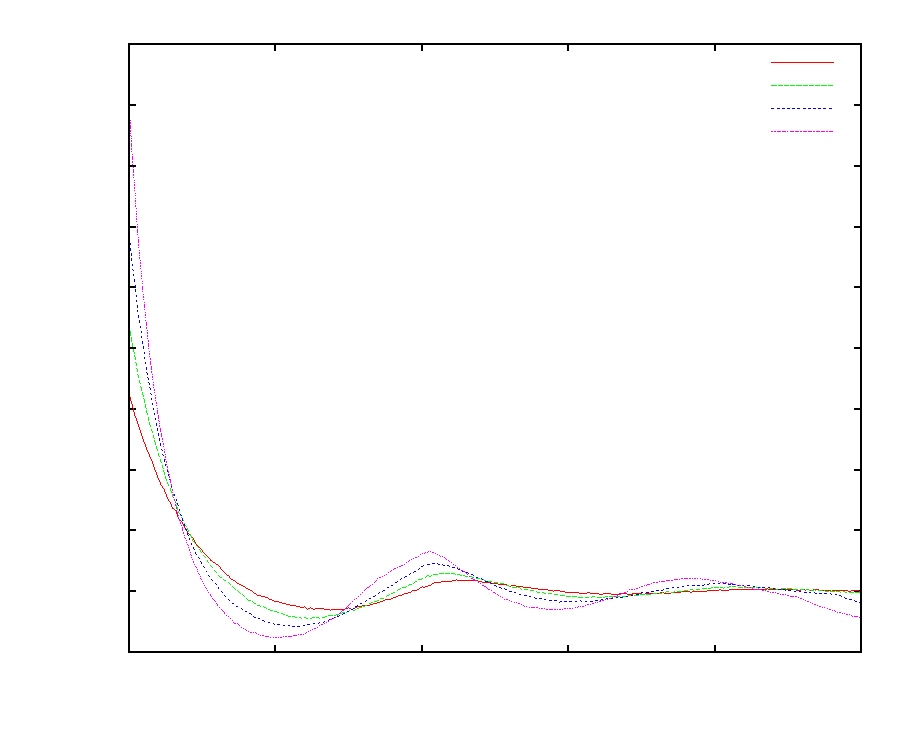
\includegraphics{PairDistribution5}}%
    \gplfronttext
  \end{picture}%
\endgroup
}
  \caption{Paarverteilungsfunktion für verschiedene Dichten $\rho$ im Bereich von 0.6 bis 0.9 (fluid) }
 \label{fig:paarverteilung2}
\end{figure} 
 
Theoretisch sollte ein System von harten Kugeln ein fcc-Kristallgitter ausbilden, dessen Gittervektoren eine relative Länge von $r_1 : r_2 : r_3 = 1 : \sqrt{2} : \sqrt{3}$ aufweisen. Bei einer Dichte von 1.3 finden sich die Maxima der Paarverteilungsfunktion auch ziemlich genau in diesen Abständen. 
 
\begin{figure}[H]
 \centering
  \resizebox{0.9\textwidth}{!}{% GNUPLOT: LaTeX picture with Postscript
\begingroup
  \makeatletter
  \providecommand\color[2][]{%
    \GenericError{(gnuplot) \space\space\space\@spaces}{%
      Package color not loaded in conjunction with
      terminal option `colourtext'%
    }{See the gnuplot documentation for explanation.%
    }{Either use 'blacktext' in gnuplot or load the package
      color.sty in LaTeX.}%
    \renewcommand\color[2][]{}%
  }%
  \providecommand\includegraphics[2][]{%
    \GenericError{(gnuplot) \space\space\space\@spaces}{%
      Package graphicx or graphics not loaded%
    }{See the gnuplot documentation for explanation.%
    }{The gnuplot epslatex terminal needs graphicx.sty or graphics.sty.}%
    \renewcommand\includegraphics[2][]{}%
  }%
  \providecommand\rotatebox[2]{#2}%
  \@ifundefined{ifGPcolor}{%
    \newif\ifGPcolor
    \GPcolortrue
  }{}%
  \@ifundefined{ifGPblacktext}{%
    \newif\ifGPblacktext
    \GPblacktextfalse
  }{}%
  % define a \g@addto@macro without @ in the name:
  \let\gplgaddtomacro\g@addto@macro
  % define empty templates for all commands taking text:
  \gdef\gplbacktext{}%
  \gdef\gplfronttext{}%
  \makeatother
  \ifGPblacktext
    % no textcolor at all
    \def\colorrgb#1{}%
    \def\colorgray#1{}%
  \else
    % gray or color?
    \ifGPcolor
      \def\colorrgb#1{\color[rgb]{#1}}%
      \def\colorgray#1{\color[gray]{#1}}%
      \expandafter\def\csname LTw\endcsname{\color{white}}%
      \expandafter\def\csname LTb\endcsname{\color{black}}%
      \expandafter\def\csname LTa\endcsname{\color{black}}%
      \expandafter\def\csname LT0\endcsname{\color[rgb]{1,0,0}}%
      \expandafter\def\csname LT1\endcsname{\color[rgb]{0,1,0}}%
      \expandafter\def\csname LT2\endcsname{\color[rgb]{0,0,1}}%
      \expandafter\def\csname LT3\endcsname{\color[rgb]{1,0,1}}%
      \expandafter\def\csname LT4\endcsname{\color[rgb]{0,1,1}}%
      \expandafter\def\csname LT5\endcsname{\color[rgb]{1,1,0}}%
      \expandafter\def\csname LT6\endcsname{\color[rgb]{0,0,0}}%
      \expandafter\def\csname LT7\endcsname{\color[rgb]{1,0.3,0}}%
      \expandafter\def\csname LT8\endcsname{\color[rgb]{0.5,0.5,0.5}}%
    \else
      % gray
      \def\colorrgb#1{\color{black}}%
      \def\colorgray#1{\color[gray]{#1}}%
      \expandafter\def\csname LTw\endcsname{\color{white}}%
      \expandafter\def\csname LTb\endcsname{\color{black}}%
      \expandafter\def\csname LTa\endcsname{\color{black}}%
      \expandafter\def\csname LT0\endcsname{\color{black}}%
      \expandafter\def\csname LT1\endcsname{\color{black}}%
      \expandafter\def\csname LT2\endcsname{\color{black}}%
      \expandafter\def\csname LT3\endcsname{\color{black}}%
      \expandafter\def\csname LT4\endcsname{\color{black}}%
      \expandafter\def\csname LT5\endcsname{\color{black}}%
      \expandafter\def\csname LT6\endcsname{\color{black}}%
      \expandafter\def\csname LT7\endcsname{\color{black}}%
      \expandafter\def\csname LT8\endcsname{\color{black}}%
    \fi
  \fi
  \setlength{\unitlength}{0.0500bp}%
  \begin{picture}(8502.00,6802.00)%
    \gplgaddtomacro\gplbacktext{%
      \csname LTb\endcsname%
      \put(814,704){\makebox(0,0)[r]{\strut{} 0}}%
      \put(814,1433){\makebox(0,0)[r]{\strut{} 2}}%
      \put(814,2162){\makebox(0,0)[r]{\strut{} 4}}%
      \put(814,2891){\makebox(0,0)[r]{\strut{} 6}}%
      \put(814,3621){\makebox(0,0)[r]{\strut{} 8}}%
      \put(814,4350){\makebox(0,0)[r]{\strut{} 10}}%
      \put(814,5079){\makebox(0,0)[r]{\strut{} 12}}%
      \put(814,5808){\makebox(0,0)[r]{\strut{} 14}}%
      \put(814,6537){\makebox(0,0)[r]{\strut{} 16}}%
      \put(946,484){\makebox(0,0){\strut{} 1}}%
      \put(2378,484){\makebox(0,0){\strut{} 1.5}}%
      \put(3810,484){\makebox(0,0){\strut{} 2}}%
      \put(5241,484){\makebox(0,0){\strut{} 2.5}}%
      \put(6673,484){\makebox(0,0){\strut{} 3}}%
      \put(8105,484){\makebox(0,0){\strut{} 3.5}}%
      \put(176,3620){\rotatebox{-270}{\makebox(0,0){\strut{}$g(r)$}}}%
      \put(4525,154){\makebox(0,0){\strut{}$r [\text{m}]$}}%
    }%
    \gplgaddtomacro\gplfronttext{%
      \csname LTb\endcsname%
      \put(7118,6364){\makebox(0,0)[r]{\strut{}$\rho$ = 1.0}}%
      \csname LTb\endcsname%
      \put(7118,6144){\makebox(0,0)[r]{\strut{}$\rho$ = 1.1}}%
      \csname LTb\endcsname%
      \put(7118,5924){\makebox(0,0)[r]{\strut{}$\rho$ = 1.2}}%
      \csname LTb\endcsname%
      \put(7118,5704){\makebox(0,0)[r]{\strut{}$\rho$ = 1.3}}%
    }%
    \gplbacktext
    \put(0,0){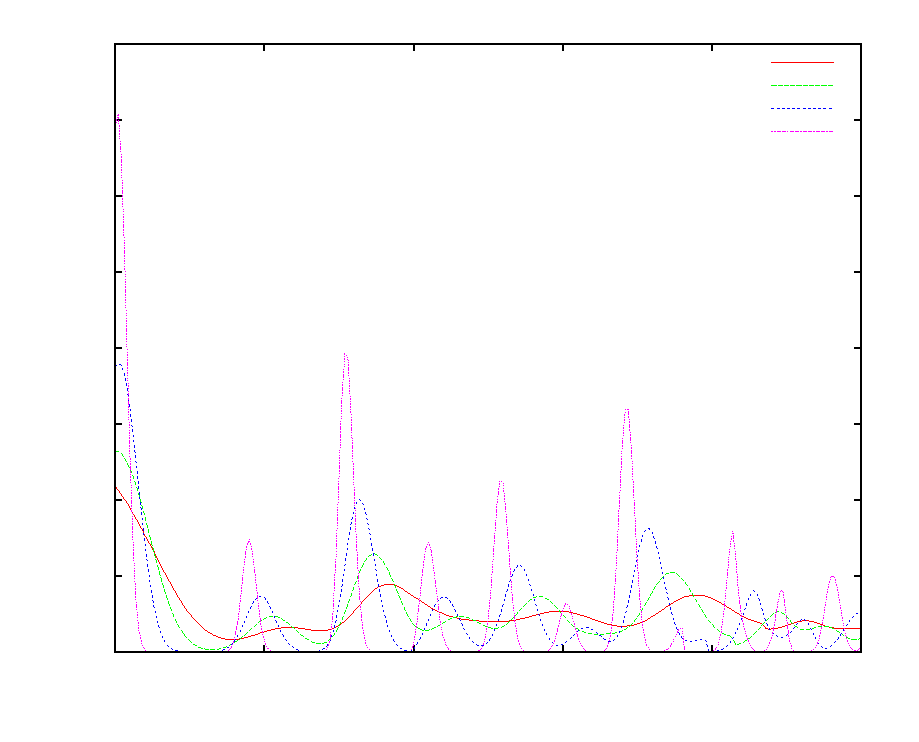
\includegraphics{PairDistribution9}}%
    \gplfronttext
  \end{picture}%
\endgroup
}
 \caption{Paarverteilungsfunktion für verschiedene Dichten $\rho$ im Bereich von 1.0 bis 1.3 (fest) }
 \label{fig:paarverteilung3}
\end{figure} 
 

\subsection{Thermische Zustandsgleichung}
Die Thermische Zustandsgleichung stellt einen Zusammenhang zwischen den Variablen Druck $p$, Temperatur $T$ und Dichte $\rho$ her. Sie kann mittels mehrerer Methoden berechnet werden. Die wohl am häufigsten verwendete bedient sich des Virials $W$  
\begin{equation}
\frac{p}{\rho k T} = 1 - \frac{1}{3NkT}\underbrace{\sum_{i=1}^N \vec{r}_i \cdot \vec{F}_i}_{= - W}
\end{equation}
Alternativ kann diese Zustandsgleichung auch geschrieben werden als 
\begin{equation}
\frac{p}{\rho k T} = 1 - \frac{2\pi\rho}{3kT} \int_0^{\infty} \text{dr} r^2 g(r) r U'(r)  
\label{eos2}
\end{equation}
Da harte Kugeln allerdings ein nicht-differenzierbares Potential besitzen und demnach keine Kraft auf sie wirkt, solange sie nicht aneinander stoßen, muss die Berechnung der Zustandsgleichung für harte Kugeln etwas abgeändert werden.
Zu diesem Zweck sieht man ein System harter Kugeln als den Grenzfall eines Systems "`weicher Kugeln"' mit dem Potential 
\begin{equation}
U_{soft}(r) = \epsilon \left(\frac{\sigma}{r}\right)^n 
\end{equation}
an, welches sich im Limes $n \rightarrow \infty$ dem Potential harter Kugeln annähert. Der Boltzmannfaktor für dieses Potential nähert sich bei $n \rightarrow \infty$ einer Stufenfunktion an
\begin{equation}
e^{-\beta U_{soft}(r)} \rightarrow H(r-\sigma)
\end{equation} 
Um die Zustandsgleichung für weiche Kugeln --- und anschließend für harte Kugeln --- herzuleiten, benötigen wir noch die formale Definition der Paarverteilungsfunktion
\begin{equation}
\rho^2 g(r_1, r_2) = N(N-1) \frac{1}{Z} \int \text{dr}_3 \ldots \text{dr}_N e^{-\beta U(r^N)}
\end{equation}
Bei additiven Paarpotentialen lässt sich der Boltzmannfaktor der Teilchen 1 und 2 aus dem Integral ziehen, da über sie nicht integriert wird, i.e. 
\begin{equation}
\rho^2 g(r_1, r_2) = e^{-\beta U(r_1, r_2)} \underbrace{N(N-1) \frac{1}{Z} \int \text{dr}_3 \ldots \text{dr}_N \exp{\left(-\beta \sum\limits_{\substack{i<j \\ i,j \neq {1,2}}} U(r^N)\right)}}_{\rho^2 y(r)}
\end{equation}
wobei der verbleibende Term $y(r)$ die Hintergrund-Korrelationsfunktion darstellt. Als Integral über zumindest stückweise stetige Funktionen --- auch im Grenzfall harter Kugeln --- ist die Hintergrund-Korrelationsfunktion selbst stetig. Die Paarverteilungsfunktion lässt sich nun wie folgt faktorisieren:
\begin{equation}
g(r) = e^{-\beta U(r)} y(r)
\label{hintergrund-korr}
\end{equation}
Dies kann nun in die Formel für die Zustandsgleichung \ref{eos2} eingesetzt werden und man gelangt zu
\begin{align*}
\frac{p}{\rho k T} &= 1 - \frac{2\pi\rho}{3kT} \int_0^{\infty} \text{dr} r^2 e^{\beta U(r)} y(r) \left[ r U'(r) \right] \\ 
&= 1 - \frac{2\pi\rho}{3kT} \int_0^{\infty} \text{dr} r^3 y(r) \frac{\text{d}}{\text{dr}} \left[ e^{-\beta U(r)} \right]
\end{align*}
Im Limes $n \rightarrow \infty$ geht die Ableitung des Boltzmannfaktors in eine Deltafunktion über und somit ergibt sich für die Zustandsgleichung harter Kugeln
\begin{equation}
\frac{p}{\rho k T} = 1 - \frac{2\pi\rho}{3kT} \sigma^3 y(\sigma) = 1 - \frac{2\pi\rho}{3kT} \sigma^3 g(\sigma)
\end{equation} 
da in diesem Grenzfall nach Gleichung \ref{hintergrund-korr} für die Paarverteilungsfunktion gilt
\begin{equation}
g(r) = H(r-\sigma)y(r) 
\end{equation}  
Die Zustandsgleichung harter Kugeln kann also über den sogenannten "`Kontaktwert"' $g(\sigma)$ der Paarverteilungsfunktion bestimmt werden. 

Eine andere Methode zur Bestimmung der Zustandsgleichung harter Kugeln ergibt sich durch Auswertung der einzelnen Kollisionen \cite{Erpenbeck1977}. Der Druck wird hierbei wie folgt berechnet: 
\begin{equation}
\frac{p}{\rho k T} = 1 + \frac{1}{t_m} \sum_{Kollisionen} \vec{r}_{ij} \cdot \Delta \vec{v}_i
\end{equation}
wobei $\vec{r}_{ij}$ die Relativposition der beiden an der Kollision beteiligten Kugeln und $\Delta \vec{v}_i$ die Änderung der Geschwindigkeit von Kugel $i$ im Verlauf der Kollision ist.
   
Abbildung \ref{fig:zustandsgleichung} zeigt die thermische Zustandsgleichung für das System aus harten Kugeln mit beiden Berechnungsmethoden. Zum Vergleich mit der Theorie ist auch die Zustandsgleichung nach Carnahan und Starling \cite{Carnahan1969} aufgetragen, welche für den stabilen fluiden Bereich gilt.
\begin{equation}
\frac{p}{\rho kT} = \frac{1 + \eta + \eta^2 -\eta^3}{(1 - \eta)^3}
\end{equation} 
wobei $\eta = \frac{\pi \rho \sigma^3}{6}$ die Packungsdichte ist. Außer für sehr geringe Dichten, stimmen Theorie und Simulation im fluiden Bereich unabhängig von der Berechnungsmethode sehr gut miteinander überein. Im festen Bereich gibt es jedoch signifikante Diskrepanzen zwischen der Berechnung über den Kontaktwert $g(\sigma)$ der Paarverteilungsfunktion und der Berechnung durch den Impulsübertrag bei Kollision.   
\begin{figure}[H]
 \centering
  \resizebox{0.9\textwidth}{!}{% GNUPLOT: LaTeX picture with Postscript
\begingroup
  \makeatletter
  \providecommand\color[2][]{%
    \GenericError{(gnuplot) \space\space\space\@spaces}{%
      Package color not loaded in conjunction with
      terminal option `colourtext'%
    }{See the gnuplot documentation for explanation.%
    }{Either use 'blacktext' in gnuplot or load the package
      color.sty in LaTeX.}%
    \renewcommand\color[2][]{}%
  }%
  \providecommand\includegraphics[2][]{%
    \GenericError{(gnuplot) \space\space\space\@spaces}{%
      Package graphicx or graphics not loaded%
    }{See the gnuplot documentation for explanation.%
    }{The gnuplot epslatex terminal needs graphicx.sty or graphics.sty.}%
    \renewcommand\includegraphics[2][]{}%
  }%
  \providecommand\rotatebox[2]{#2}%
  \@ifundefined{ifGPcolor}{%
    \newif\ifGPcolor
    \GPcolortrue
  }{}%
  \@ifundefined{ifGPblacktext}{%
    \newif\ifGPblacktext
    \GPblacktextfalse
  }{}%
  % define a \g@addto@macro without @ in the name:
  \let\gplgaddtomacro\g@addto@macro
  % define empty templates for all commands taking text:
  \gdef\gplbacktext{}%
  \gdef\gplfronttext{}%
  \makeatother
  \ifGPblacktext
    % no textcolor at all
    \def\colorrgb#1{}%
    \def\colorgray#1{}%
  \else
    % gray or color?
    \ifGPcolor
      \def\colorrgb#1{\color[rgb]{#1}}%
      \def\colorgray#1{\color[gray]{#1}}%
      \expandafter\def\csname LTw\endcsname{\color{white}}%
      \expandafter\def\csname LTb\endcsname{\color{black}}%
      \expandafter\def\csname LTa\endcsname{\color{black}}%
      \expandafter\def\csname LT0\endcsname{\color[rgb]{1,0,0}}%
      \expandafter\def\csname LT1\endcsname{\color[rgb]{0,1,0}}%
      \expandafter\def\csname LT2\endcsname{\color[rgb]{0,0,1}}%
      \expandafter\def\csname LT3\endcsname{\color[rgb]{1,0,1}}%
      \expandafter\def\csname LT4\endcsname{\color[rgb]{0,1,1}}%
      \expandafter\def\csname LT5\endcsname{\color[rgb]{1,1,0}}%
      \expandafter\def\csname LT6\endcsname{\color[rgb]{0,0,0}}%
      \expandafter\def\csname LT7\endcsname{\color[rgb]{1,0.3,0}}%
      \expandafter\def\csname LT8\endcsname{\color[rgb]{0.5,0.5,0.5}}%
    \else
      % gray
      \def\colorrgb#1{\color{black}}%
      \def\colorgray#1{\color[gray]{#1}}%
      \expandafter\def\csname LTw\endcsname{\color{white}}%
      \expandafter\def\csname LTb\endcsname{\color{black}}%
      \expandafter\def\csname LTa\endcsname{\color{black}}%
      \expandafter\def\csname LT0\endcsname{\color{black}}%
      \expandafter\def\csname LT1\endcsname{\color{black}}%
      \expandafter\def\csname LT2\endcsname{\color{black}}%
      \expandafter\def\csname LT3\endcsname{\color{black}}%
      \expandafter\def\csname LT4\endcsname{\color{black}}%
      \expandafter\def\csname LT5\endcsname{\color{black}}%
      \expandafter\def\csname LT6\endcsname{\color{black}}%
      \expandafter\def\csname LT7\endcsname{\color{black}}%
      \expandafter\def\csname LT8\endcsname{\color{black}}%
    \fi
  \fi
  \setlength{\unitlength}{0.0500bp}%
  \begin{picture}(8502.00,6802.00)%
    \gplgaddtomacro\gplbacktext{%
      \csname LTb\endcsname%
      \put(814,704){\makebox(0,0)[r]{\strut{} 0}}%
      \put(814,1676){\makebox(0,0)[r]{\strut{} 5}}%
      \put(814,2648){\makebox(0,0)[r]{\strut{} 10}}%
      \put(814,3621){\makebox(0,0)[r]{\strut{} 15}}%
      \put(814,4593){\makebox(0,0)[r]{\strut{} 20}}%
      \put(814,5565){\makebox(0,0)[r]{\strut{} 25}}%
      \put(814,6537){\makebox(0,0)[r]{\strut{} 30}}%
      \put(946,484){\makebox(0,0){\strut{} 0.2}}%
      \put(2139,484){\makebox(0,0){\strut{} 0.4}}%
      \put(3332,484){\makebox(0,0){\strut{} 0.6}}%
      \put(4526,484){\makebox(0,0){\strut{} 0.8}}%
      \put(5719,484){\makebox(0,0){\strut{} 1}}%
      \put(6912,484){\makebox(0,0){\strut{} 1.2}}%
      \put(8105,484){\makebox(0,0){\strut{} 1.4}}%
      \put(176,3620){\rotatebox{-270}{\makebox(0,0){\strut{}$p/\rho k T$}}}%
      \put(4525,154){\makebox(0,0){\strut{}$
\rho [\text{m}^{-3}]$}}%
    }%
    \gplgaddtomacro\gplfronttext{%
      \csname LTb\endcsname%
      \put(7118,6364){\makebox(0,0)[r]{\strut{}aus Paarverteilungsfunktion}}%
      \csname LTb\endcsname%
      \put(7118,6144){\makebox(0,0)[r]{\strut{}aus Impulsübertrag}}%
      \csname LTb\endcsname%
      \put(7118,5924){\makebox(0,0)[r]{\strut{}Theorie}}%
    }%
    \gplbacktext
    \put(0,0){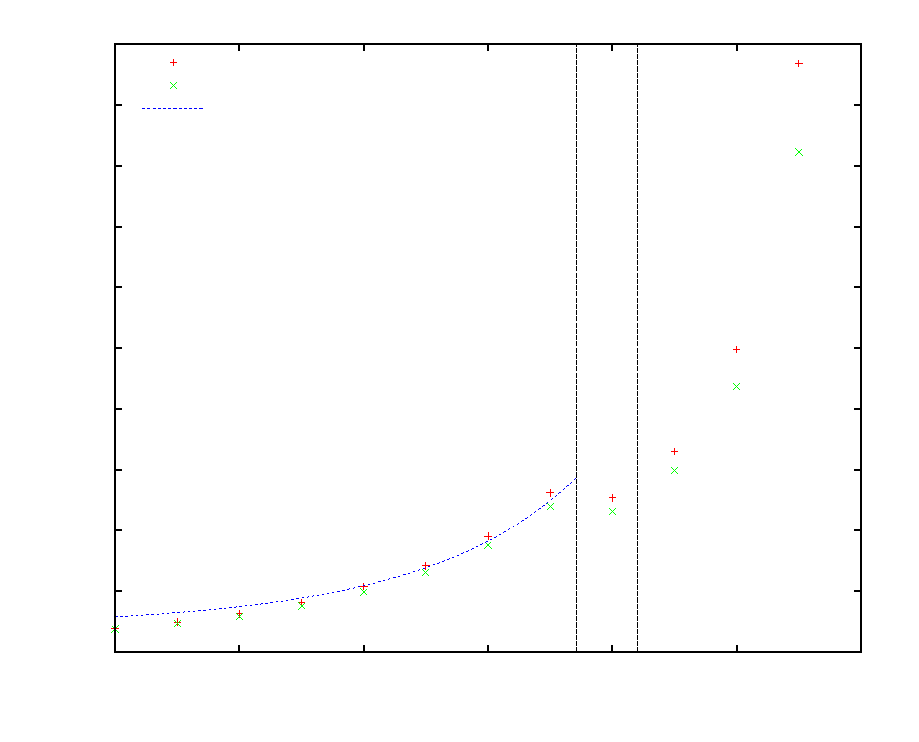
\includegraphics{eos}}%
    \gplfronttext
  \end{picture}%
\endgroup
}
 \caption{Thermische Zustandsgleichung des Systems aus harten Kugeln}
 \label{fig:zustandsgleichung}
\end{figure} 


\subsection{Diffusion}
Des weiteren wurde die Diffusionskonstante $D$ für verschiedene Werte der Dichte $\rho$ berechnet. Sie ergibt sich nach der Green-Kubo-Relation aus dem Intgral über die Geschwindigkeits-Autokorrelationsfunktion $C(t)$.
\begin{equation}
D = \frac{1}{3}\int_0^{\infty} \langle \vec{v}_i(0)\cdot \vec{v}_i(t)\rangle \text{dt}
\end{equation}
Zum Vergleich wurde die empirische Formel von Speedy \cite{Speedy1987} herangezogen.
\begin{equation}
D = \frac{D_0}{\rho^*}\left(1-\frac{\rho^*}{1.09}\right)\left(1+\rho^{*2}\left(0.4 - 0.83\rho^{*2}\right)\right)
\end{equation}
wobei $\rho^*= \rho \sigma^3$ die reduzierte Dichte ist und $D_0 = \frac{3}{8} \sigma \left(\frac{kT}{\pi m}\right)^{\frac{1}{2}}$. Abbildung \ref{fig:diffusion} zeigt die Diffusionskonstante bei harten Kugeln. Es zeigt sich eine gute Übereinstimmung mit den Ergebnissen von Speedy \cite{Speedy1987}.
\begin{figure}[H]
 \centering
  \resizebox{0.9\textwidth}{!}{% GNUPLOT: LaTeX picture with Postscript
\begingroup
  \makeatletter
  \providecommand\color[2][]{%
    \GenericError{(gnuplot) \space\space\space\@spaces}{%
      Package color not loaded in conjunction with
      terminal option `colourtext'%
    }{See the gnuplot documentation for explanation.%
    }{Either use 'blacktext' in gnuplot or load the package
      color.sty in LaTeX.}%
    \renewcommand\color[2][]{}%
  }%
  \providecommand\includegraphics[2][]{%
    \GenericError{(gnuplot) \space\space\space\@spaces}{%
      Package graphicx or graphics not loaded%
    }{See the gnuplot documentation for explanation.%
    }{The gnuplot epslatex terminal needs graphicx.sty or graphics.sty.}%
    \renewcommand\includegraphics[2][]{}%
  }%
  \providecommand\rotatebox[2]{#2}%
  \@ifundefined{ifGPcolor}{%
    \newif\ifGPcolor
    \GPcolortrue
  }{}%
  \@ifundefined{ifGPblacktext}{%
    \newif\ifGPblacktext
    \GPblacktextfalse
  }{}%
  % define a \g@addto@macro without @ in the name:
  \let\gplgaddtomacro\g@addto@macro
  % define empty templates for all commands taking text:
  \gdef\gplbacktext{}%
  \gdef\gplfronttext{}%
  \makeatother
  \ifGPblacktext
    % no textcolor at all
    \def\colorrgb#1{}%
    \def\colorgray#1{}%
  \else
    % gray or color?
    \ifGPcolor
      \def\colorrgb#1{\color[rgb]{#1}}%
      \def\colorgray#1{\color[gray]{#1}}%
      \expandafter\def\csname LTw\endcsname{\color{white}}%
      \expandafter\def\csname LTb\endcsname{\color{black}}%
      \expandafter\def\csname LTa\endcsname{\color{black}}%
      \expandafter\def\csname LT0\endcsname{\color[rgb]{1,0,0}}%
      \expandafter\def\csname LT1\endcsname{\color[rgb]{0,1,0}}%
      \expandafter\def\csname LT2\endcsname{\color[rgb]{0,0,1}}%
      \expandafter\def\csname LT3\endcsname{\color[rgb]{1,0,1}}%
      \expandafter\def\csname LT4\endcsname{\color[rgb]{0,1,1}}%
      \expandafter\def\csname LT5\endcsname{\color[rgb]{1,1,0}}%
      \expandafter\def\csname LT6\endcsname{\color[rgb]{0,0,0}}%
      \expandafter\def\csname LT7\endcsname{\color[rgb]{1,0.3,0}}%
      \expandafter\def\csname LT8\endcsname{\color[rgb]{0.5,0.5,0.5}}%
    \else
      % gray
      \def\colorrgb#1{\color{black}}%
      \def\colorgray#1{\color[gray]{#1}}%
      \expandafter\def\csname LTw\endcsname{\color{white}}%
      \expandafter\def\csname LTb\endcsname{\color{black}}%
      \expandafter\def\csname LTa\endcsname{\color{black}}%
      \expandafter\def\csname LT0\endcsname{\color{black}}%
      \expandafter\def\csname LT1\endcsname{\color{black}}%
      \expandafter\def\csname LT2\endcsname{\color{black}}%
      \expandafter\def\csname LT3\endcsname{\color{black}}%
      \expandafter\def\csname LT4\endcsname{\color{black}}%
      \expandafter\def\csname LT5\endcsname{\color{black}}%
      \expandafter\def\csname LT6\endcsname{\color{black}}%
      \expandafter\def\csname LT7\endcsname{\color{black}}%
      \expandafter\def\csname LT8\endcsname{\color{black}}%
    \fi
  \fi
  \setlength{\unitlength}{0.0500bp}%
  \begin{picture}(8502.00,6802.00)%
    \gplgaddtomacro\gplbacktext{%
      \csname LTb\endcsname%
      \put(946,704){\makebox(0,0)[r]{\strut{}-0.1}}%
      \put(946,1287){\makebox(0,0)[r]{\strut{} 0}}%
      \put(946,1871){\makebox(0,0)[r]{\strut{} 0.1}}%
      \put(946,2454){\makebox(0,0)[r]{\strut{} 0.2}}%
      \put(946,3037){\makebox(0,0)[r]{\strut{} 0.3}}%
      \put(946,3621){\makebox(0,0)[r]{\strut{} 0.4}}%
      \put(946,4204){\makebox(0,0)[r]{\strut{} 0.5}}%
      \put(946,4787){\makebox(0,0)[r]{\strut{} 0.6}}%
      \put(946,5370){\makebox(0,0)[r]{\strut{} 0.7}}%
      \put(946,5954){\makebox(0,0)[r]{\strut{} 0.8}}%
      \put(946,6537){\makebox(0,0)[r]{\strut{} 0.9}}%
      \put(1078,484){\makebox(0,0){\strut{} 0.2}}%
      \put(2249,484){\makebox(0,0){\strut{} 0.4}}%
      \put(3420,484){\makebox(0,0){\strut{} 0.6}}%
      \put(4592,484){\makebox(0,0){\strut{} 0.8}}%
      \put(5763,484){\makebox(0,0){\strut{} 1}}%
      \put(6934,484){\makebox(0,0){\strut{} 1.2}}%
      \put(8105,484){\makebox(0,0){\strut{} 1.4}}%
      \put(176,3620){\rotatebox{-270}{\makebox(0,0){\strut{}$D$}}}%
      \put(4591,154){\makebox(0,0){\strut{}$\rho $}}%
    }%
    \gplgaddtomacro\gplfronttext{%
      \csname LTb\endcsname%
      \put(7118,6364){\makebox(0,0)[r]{\strut{}Simulation}}%
      \csname LTb\endcsname%
      \put(7118,6144){\makebox(0,0)[r]{\strut{}Theorie}}%
    }%
    \gplbacktext
    \put(0,0){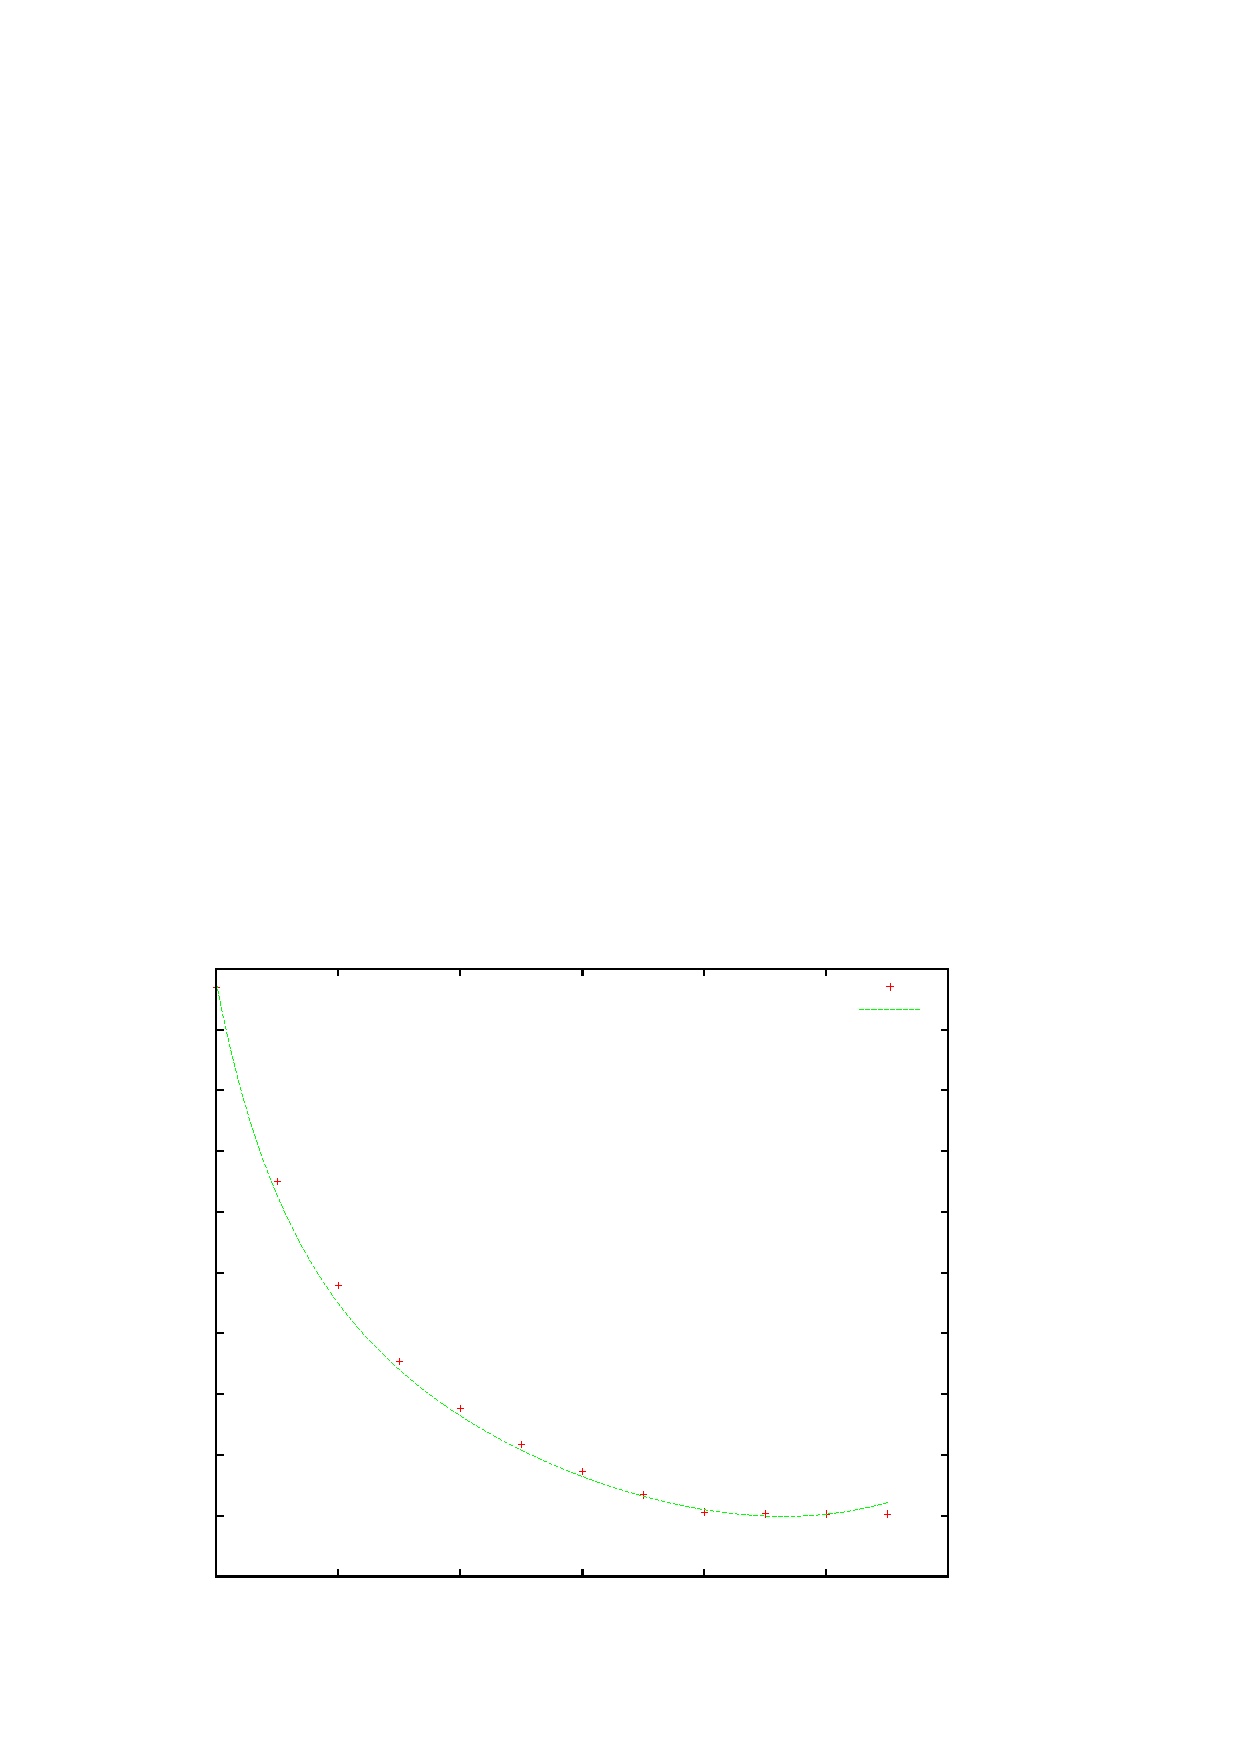
\includegraphics{diffusion}}%
    \gplfronttext
  \end{picture}%
\endgroup
}
 \caption{Diffusionskonstante bei harten Kugeln}
 \label{fig:diffusion}
\end{figure} 

\subsection{Freie Bewegungszeiten}
Anschließend wurden noch die freien Bewegungszeiten --- also die Zeiten zwischen zwei Stößen --- untersucht und deren Wahrscheinlichkeitsverteilung analysiert. Bei geringen Dichten kann man molekulares Chaos annehmen und kommt somit zu dem Schluss, dass die Wahrscheinlichkeitsverteilung $p(\tau)$ einem exponentiellen Abfall folgt.
\begin{equation}
p(\tau) = c\cdot e^{-\frac{\tau}{\tau_0}}
\end{equation} 
wobei $c$ nur eine Normierungskonstante ist, sodass $\int_0^{\infty} p(\tau) \text{d}\tau = 1$. Um dies zu überprüfen und den Parameter $\tau_0$ zu bestimmen, welcher von der Dichte $\rho$ abhängt, wurde der Logarithmus der Wahrscheinlichkeitsverteilung $p(\tau)$ an eine lineare Funktion $f(\tau) = a\cdot \tau + b$ angepasst. Abbildung \ref{fig:flight} zeigt den so berechneten Parameter $\tau_0$ in Abhängigkeit von der Dichte $\rho$. Statt $\tau_0$ wurde allerdings sein Inverses aufgetragen, da sich hier eine annähernd lineare Abhängigkeit von der Dichte im Bereich verdünnter (fluider) Systeme zeigt. Dies ist im Einklang mit den Resultaten von Wiegel und Michels \cite{Wiegel1979}. 

\begin{figure}[H]
 \centering
  \resizebox{0.9\textwidth}{!}{% GNUPLOT: LaTeX picture with Postscript
\begingroup
  \makeatletter
  \providecommand\color[2][]{%
    \GenericError{(gnuplot) \space\space\space\@spaces}{%
      Package color not loaded in conjunction with
      terminal option `colourtext'%
    }{See the gnuplot documentation for explanation.%
    }{Either use 'blacktext' in gnuplot or load the package
      color.sty in LaTeX.}%
    \renewcommand\color[2][]{}%
  }%
  \providecommand\includegraphics[2][]{%
    \GenericError{(gnuplot) \space\space\space\@spaces}{%
      Package graphicx or graphics not loaded%
    }{See the gnuplot documentation for explanation.%
    }{The gnuplot epslatex terminal needs graphicx.sty or graphics.sty.}%
    \renewcommand\includegraphics[2][]{}%
  }%
  \providecommand\rotatebox[2]{#2}%
  \@ifundefined{ifGPcolor}{%
    \newif\ifGPcolor
    \GPcolortrue
  }{}%
  \@ifundefined{ifGPblacktext}{%
    \newif\ifGPblacktext
    \GPblacktextfalse
  }{}%
  % define a \g@addto@macro without @ in the name:
  \let\gplgaddtomacro\g@addto@macro
  % define empty templates for all commands taking text:
  \gdef\gplbacktext{}%
  \gdef\gplfronttext{}%
  \makeatother
  \ifGPblacktext
    % no textcolor at all
    \def\colorrgb#1{}%
    \def\colorgray#1{}%
  \else
    % gray or color?
    \ifGPcolor
      \def\colorrgb#1{\color[rgb]{#1}}%
      \def\colorgray#1{\color[gray]{#1}}%
      \expandafter\def\csname LTw\endcsname{\color{white}}%
      \expandafter\def\csname LTb\endcsname{\color{black}}%
      \expandafter\def\csname LTa\endcsname{\color{black}}%
      \expandafter\def\csname LT0\endcsname{\color[rgb]{1,0,0}}%
      \expandafter\def\csname LT1\endcsname{\color[rgb]{0,1,0}}%
      \expandafter\def\csname LT2\endcsname{\color[rgb]{0,0,1}}%
      \expandafter\def\csname LT3\endcsname{\color[rgb]{1,0,1}}%
      \expandafter\def\csname LT4\endcsname{\color[rgb]{0,1,1}}%
      \expandafter\def\csname LT5\endcsname{\color[rgb]{1,1,0}}%
      \expandafter\def\csname LT6\endcsname{\color[rgb]{0,0,0}}%
      \expandafter\def\csname LT7\endcsname{\color[rgb]{1,0.3,0}}%
      \expandafter\def\csname LT8\endcsname{\color[rgb]{0.5,0.5,0.5}}%
    \else
      % gray
      \def\colorrgb#1{\color{black}}%
      \def\colorgray#1{\color[gray]{#1}}%
      \expandafter\def\csname LTw\endcsname{\color{white}}%
      \expandafter\def\csname LTb\endcsname{\color{black}}%
      \expandafter\def\csname LTa\endcsname{\color{black}}%
      \expandafter\def\csname LT0\endcsname{\color{black}}%
      \expandafter\def\csname LT1\endcsname{\color{black}}%
      \expandafter\def\csname LT2\endcsname{\color{black}}%
      \expandafter\def\csname LT3\endcsname{\color{black}}%
      \expandafter\def\csname LT4\endcsname{\color{black}}%
      \expandafter\def\csname LT5\endcsname{\color{black}}%
      \expandafter\def\csname LT6\endcsname{\color{black}}%
      \expandafter\def\csname LT7\endcsname{\color{black}}%
      \expandafter\def\csname LT8\endcsname{\color{black}}%
    \fi
  \fi
  \setlength{\unitlength}{0.0500bp}%
  \begin{picture}(8502.00,6802.00)%
    \gplgaddtomacro\gplbacktext{%
      \csname LTb\endcsname%
      \put(1078,704){\makebox(0,0)[r]{\strut{} 0}}%
      \put(1078,1287){\makebox(0,0)[r]{\strut{} 500}}%
      \put(1078,1871){\makebox(0,0)[r]{\strut{} 1000}}%
      \put(1078,2454){\makebox(0,0)[r]{\strut{} 1500}}%
      \put(1078,3037){\makebox(0,0)[r]{\strut{} 2000}}%
      \put(1078,3621){\makebox(0,0)[r]{\strut{} 2500}}%
      \put(1078,4204){\makebox(0,0)[r]{\strut{} 3000}}%
      \put(1078,4787){\makebox(0,0)[r]{\strut{} 3500}}%
      \put(1078,5370){\makebox(0,0)[r]{\strut{} 4000}}%
      \put(1078,5954){\makebox(0,0)[r]{\strut{} 4500}}%
      \put(1078,6537){\makebox(0,0)[r]{\strut{} 5000}}%
      \put(1837,484){\makebox(0,0){\strut{} 0.2}}%
      \put(3090,484){\makebox(0,0){\strut{} 0.4}}%
      \put(4344,484){\makebox(0,0){\strut{} 0.6}}%
      \put(5598,484){\makebox(0,0){\strut{} 0.8}}%
      \put(6851,484){\makebox(0,0){\strut{} 1}}%
      \put(8105,484){\makebox(0,0){\strut{} 1.2}}%
      \put(176,3620){\rotatebox{-270}{\makebox(0,0){\strut{}$1/\tau_0$}}}%
      \put(4657,154){\makebox(0,0){\strut{}$\rho$}}%
    }%
    \gplgaddtomacro\gplfronttext{%
    }%
    \gplbacktext
    \put(0,0){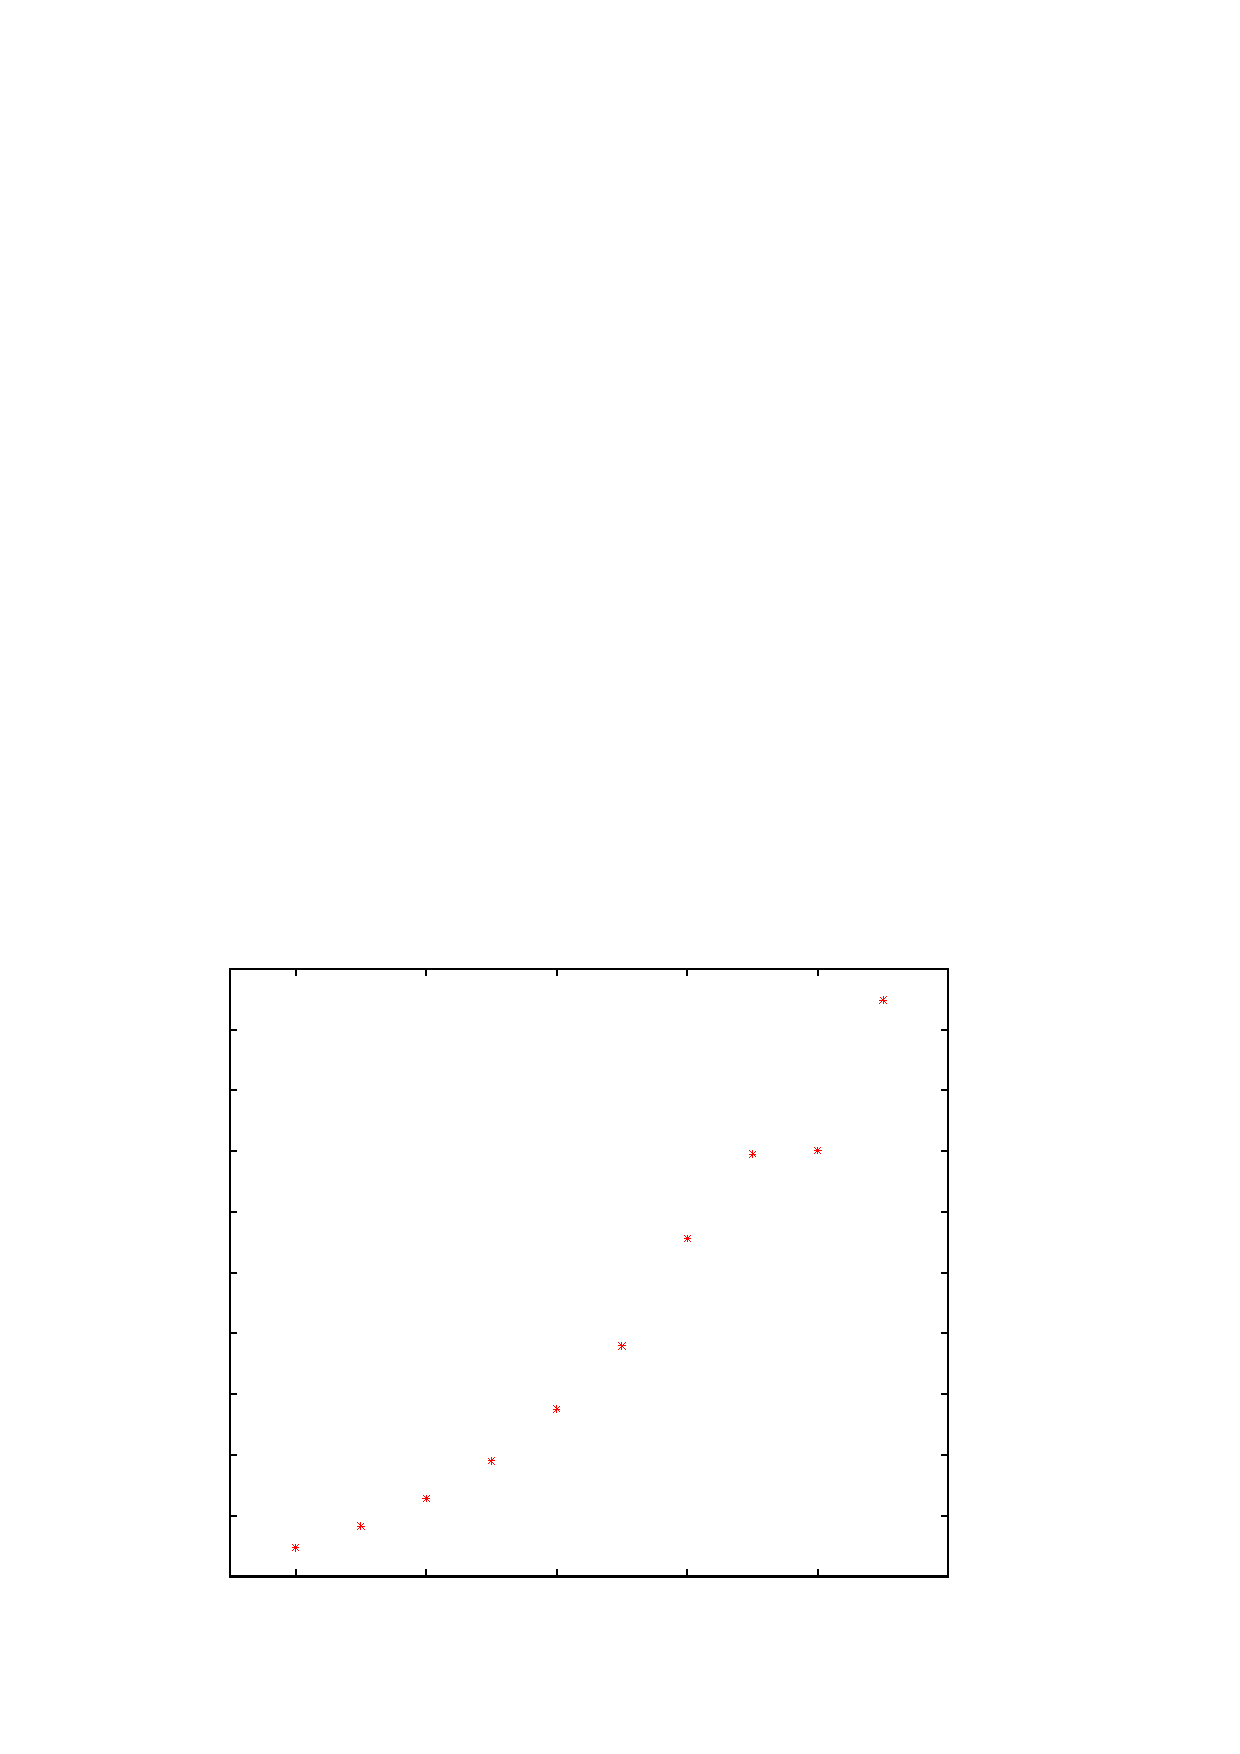
\includegraphics{flight_fit_inverse}}%
    \gplfronttext
  \end{picture}%
\endgroup
}
 \caption{Durch linearen Fit bestimmte Konstante $\tau_0$ in Abhängigkeit von $\rho$}
 \label{fig:flight}
\end{figure} 

\section{Conclusio} \label{conclusio}
% !TeX root = ../Harte_Kugeln.tex
Innerhalb dieses Projekts im Rahmen des Praktikums ``Computational Physics'' ist es uns gelungen, einige Eigenschaften eines Systems harter Kugeln mit Hilfe von ereignisbasierter Molekulardynamik zu bestimmen. Die gefundenen Resultate wie Paarverteilungsfunktion, Diffusionskonstante und freie Bewegungszeiten bei verschiedenen Dichten sowie auch die thermische Zustandsgleichung stimmen weitgehend mit bereits publizierten theoretischen und simulationsgestützten Ergebnissen überein.  



\bibliographystyle{IEEEtran} % kürzt automatisch vornamen ab und so zeug 
\bibliography{../biblio}
\end{document}